%Beamer class
\documentclass{beamer}

\usepackage[czech]{babel}
\usepackage[cp1250]{inputenc}
\usepackage{fontenc}
\usepackage{tgheros}
\usepackage{array}
\usepackage{color}
\usepackage{hyperref}

\usetheme{Antibes}
\usecolortheme{crane}


\title[BE1M13VES]{BE1M13VES}
\subtitle[Manufacturing of Electrical Components] {Manufacturing of Electrical Components}
\author[Brejcha]{Michal Brejcha}
\institute[CTU]{CTU in Prague}
\date[Prague, 2017]{Prague, 2017}

\begin{document}
%------------------------------------------------------------------------------
%Uvodni slajd
%------------------------------------------------------------------------------
\frame{\titlepage}

\begin{frame}
\frametitle{Overview} 
\tableofcontents
\end{frame}

\AtBeginSection[]
{
  \begin{frame}
    \frametitle{TOPIC}
    \tableofcontents[currentsection]
  \end{frame}
}

%------------------------------------------------------------------------------
%Capacitance
%------------------------------------------------------------------------------
\section{\texorpdfstring{Inductance}{Inductance}}
%------------------------------------------------------------------------------
	\begin{frame}
    \frametitle{Inductors}
		
		\begin{itemize}
			\item Devices with the lowest portfolio on the market, very pure mass-production. 
			\item Often must be inductance designed \uv{on-demand} during designing process.
		\end{itemize}
		\textbf{Types according to the design:}
		
		\begin{itemize}
			\item coils without magnetic core (air-wounded)
			\item coils with ferromagnetic core:
			\begin{itemize}
				\item polycrystalline - printed cores, powder cores,
				\item amorphous cores - magnetic glasses, oxides (ferrite - Manganese + Zinc, Nickel + Zinc)
			\end{itemize}
		\end{itemize}
  \end{frame}
%------------------------------------------------------------------------------
	\begin{frame}
    \frametitle{Inductors - parameters}
		\begin{tabular}{p{0.25\linewidth} p{0.65\linewidth}}
		\textbf{Parameters:} &
		\begin{itemize}
			\item $L$... inductance (H)
			\item $I$... nominal current (A)
			\item $Q$... quality factor (-)
			\item ... temperature dependence
			\item ... current and voltage dependence
			\item ... frequency dependence
		\end{itemize} \\
		\textbf{Quantities} &
		\begin{itemize}
			\item $B$... magnetic flux density (T)
			\item $H$... magnetic excitation (A/m)
			\item $\phi$... magnetic flux (Wb)
			\item $\mu$... permeability (H/m)
		\end{itemize}
		\end{tabular}
  \end{frame}
%------------------------------------------------------------------------------
	\begin{frame}
    \frametitle{Inductance Calculation}
		There is no typical topology for inductance calculation. The resulting formulas can be quite complicated. There are three definitions of inductance:
		\begin{tabular}{m{0.4\linewidth} m{0.5\linewidth}}
		\begin{enumerate}
			\item Static definition: $$N\cdot \phi(t)= L\cdot i(t)$$
			\item Dynamic definition: $$u_i(t)=-L\cdot \frac{\partial i(t)}{\partial t}$$
			\item Energy definition: $$E_L= \frac{1}{2}\cdot L\cdot I^2$$
		\end{enumerate}
		& 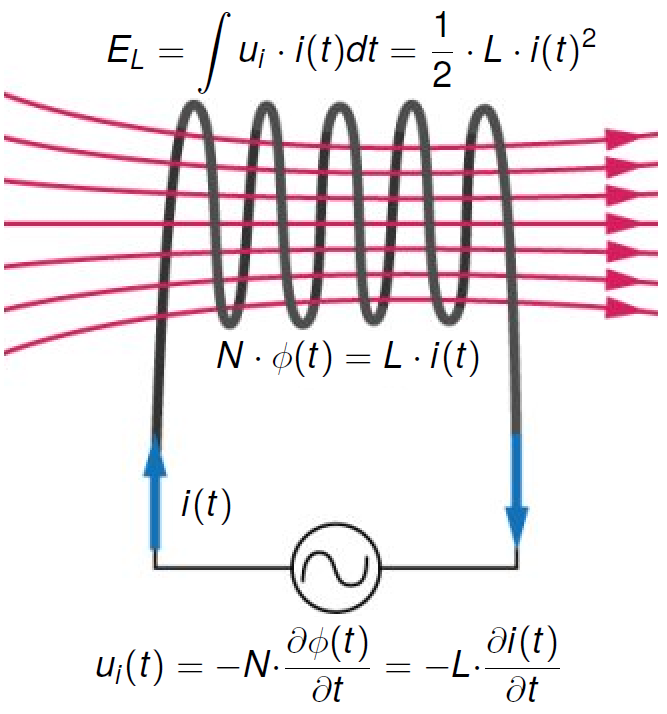
\includegraphics[scale=0.28]{obr01_defIndukcnosti.png}
		\end{tabular}
	\end{frame}
%------------------------------------------------------------------------------
	\begin{frame}
	\frametitle{Inductance of coils with ferromagnetic cores}
	Inductance is very often computed via core constant $A_L$
	$$\oint H dx = N\cdot I \Rightarrow H\cdot d_S = N\cdot I$$
		\begin{tabular}{m{0.3\linewidth} m{0.6\linewidth}}
		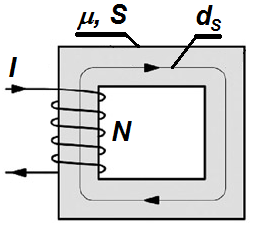
\includegraphics[scale=0.48]{obr02_mgObvod.png} & 
		$$B = N\cdot I\cdot \frac{\mu}{d_S}\Rightarrow \phi= N\cdot I\cdot \frac{\mu\cdot S}{d_S}$$
		Then for inductance:
		$$L= \frac{N^2\cdot\mu\cdot S}{d_S} = N^2 \cdot A_L$$
		\end{tabular}
  \end{frame}
%------------------------------------------------------------------------------
	\begin{frame}
	\frametitle{Inductance of air coils}
	Inductance is primary given by a geometric shape and dimensions of coil and by the number of turns ($N$). For design and computing are often used empiric formulas, e.g. Nagaoko's formula:
	$$L= 0.03948\cdot \frac{D^2\cdot N^2\cdot K}{4\cdot L}$$
	\small
		\begin{tabular}{m{0.3\linewidth} m{0.6\linewidth}}
		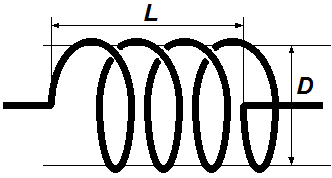
\includegraphics[scale=0.35]{obr03_vzdInduk.png} & 
		\begin{tabular}{|c|c|c|c|c|}
		\hline
		\textbf{D/L} & 0.00 & 0.25 & 0.50 & 0.75 \\
		\hline
		\textbf{K}   & 1.000 & 0.902 & 0.818 & 0.748 \\
		\hline\hline
		\textbf{D/L} & 1.00 & 1.25 & 1.50 & 2.00 \\
		\hline
		\textbf{K}   & 0.688 & 0.638 & 0.595 & 0.525 \\
		\hline\hline
		\textbf{D/L} & 2.50 & 3.00 & 3.50 & 4.00 \\
		\hline
		\textbf{K}   & 0.472 & 0.429 & 0.394 & 0.365 \\
		\hline
		\end{tabular}
		\end{tabular}
  \end{frame}
%------------------------------------------------------------------------------
	\begin{frame}
	\frametitle{Inductance of air coils}
	\begin{flushleft}
		$L$ is inductance ($\mu H$), $D$ ($cm$) is a diameter of coil, $l$ ($cm$) is the length of coil and $K$ is a ration coefficient from the table. 
	\end{flushleft}
	\begin{flushleft}
		For preliminary estimation of inductance can be used another simplified formula: ($nH$; $cm$) 
	\end{flushleft}
	$$L=\frac{\pi^2\cdot N^2 \cdot D^2}{1+0.4\cdot D}$$
  \end{frame}
%------------------------------------------------------------------------------
%Technology
%------------------------------------------------------------------------------
\section{\texorpdfstring{Technology}{Technology}}
%------------------------------------------------------------------------------
	\begin{frame}
	\frametitle{Coils without Core (Air)}
	\begin{center}
		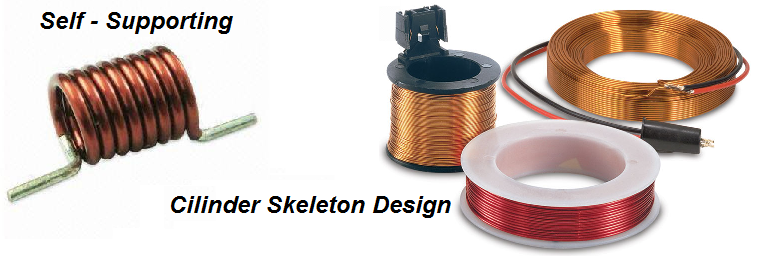
\includegraphics[scale=0.45]{obr04_vzdCivky.png}
	\end{center}
	\small
	\begin{itemize}
		\item coils with relatively low inductance (as small as 100~nH up to 1~mH), 
		\item stable parameters and quite linear characteristics,
		\item ideal for low-power and high frequency applications, 
		\item the design (diameter, wire surface...) is affected by quality factor requirements.
	\end{itemize}
  \end{frame}
%------------------------------------------------------------------------------
	\begin{frame}
	\frametitle{Air Coils - Winding}
	\begin{itemize}
		\item Single or multi-layer winding made from a wire with rounded or square cross-section, 
		\item windings are sometimes separated into chambers (sectors), especially for minimizing self-capacity,
		\item for high frequency (about 50 kHz) is sometimes used basket winding.
		\begin{itemize}
			\item Smaller \textcolor{blue}{proximity effect},
			\item smaller self capacitance.
		\end{itemize}
	\end{itemize}
  \end{frame}
%------------------------------------------------------------------------------
	\begin{frame}
	\frametitle{Air Coils - Winding}
	\begin{center}
		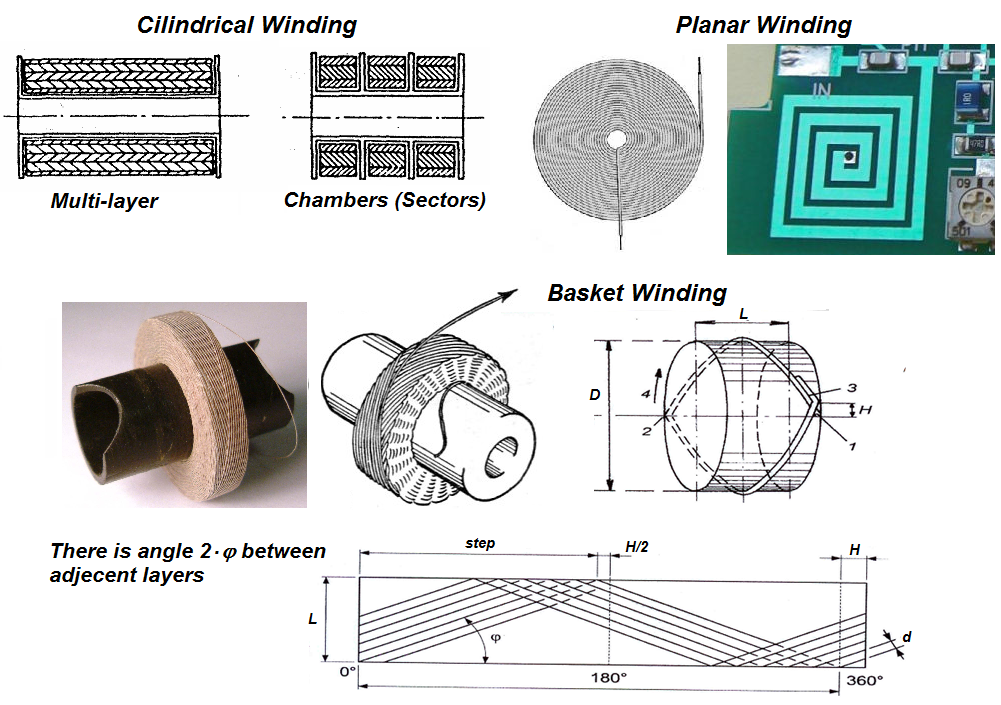
\includegraphics[scale=0.35]{obr05_vzdVinuti.png}
	\end{center}
  \end{frame}
%------------------------------------------------------------------------------
	\begin{frame}
	\frametitle{Design Example - Resonator}
	\small
	\begin{flushleft}
		For high quality factor, wire must have very low resistance. Quality factor is nearly proportional to dimensions (volume) of a coil. Optimum of coil length is in the range from $0,5\cdot D$ up to $D$ ($D$ is the diameter).
	\end{flushleft}
	\begin{flushleft}
		The quality factor is affected by the \textcolor{blue}{skin effect} at the high frequencies: $$\delta = \sqrt{\frac{2}{\omega\cdot \mu\cdot \sigma}}$$
	\end{flushleft}
	\begin{center}
		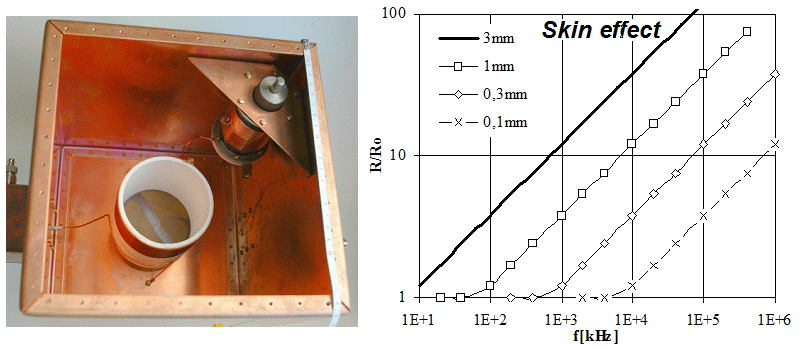
\includegraphics[scale=0.35]{obr06_Papez.png}
	\end{center}
  \end{frame}
%------------------------------------------------------------------------------
	\begin{frame}
	\frametitle{Coils with Ferromagnetic Cores}
		\small
	\textbf{Cores} are used to increase the inductance (they have higher permeability $\mu$). Disadvantages:
	\begin{tabular}{m{0.45\linewidth} m{0.45\linewidth}}
	\begin{itemize}
		\item non-linearity
		\item frequency dependence
		\item power-losses
		\begin{itemize}
			\item hysteresis losses $$\frac{P_h}{V} \approx 2\cdot f\cdot B_m\cdot H_C \approx  2\cdot f\cdot B_m^\alpha$$
			\item eddy currents $$\frac{P_{ed}}{V} \approx \pi\cdot f^2\cdot B_m^2\cdot d^2 $$
		\end{itemize}
	\end{itemize}
	&
	\begin{description}
		\item[$V$]... volume,
	  \item[$f$]... frequency,
		\item[$B_m$]... mag. flux density (maximum),
		\item[$H_C$]... coercivity,
		\item[$d$]... thickness of the material,
		\item[$\alpha$]... approximation exponent ($\approx 2$)
	\end{description}
	\end{tabular}
  \end{frame}
%------------------------------------------------------------------------------
	\begin{frame}
	\frametitle{Cores - Examples}
	\begin{center}
		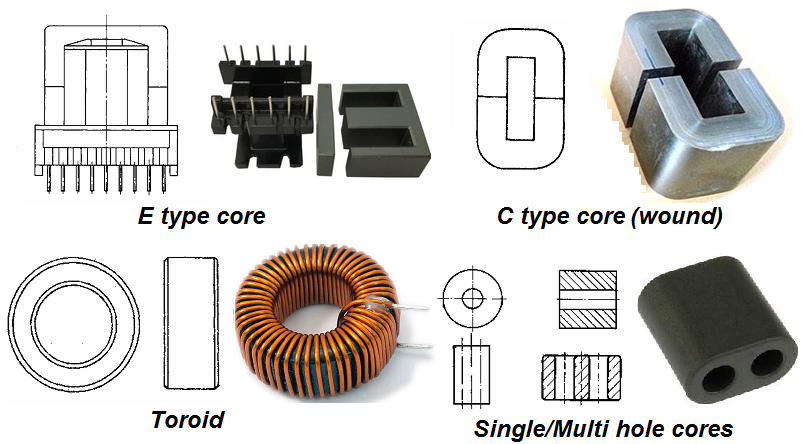
\includegraphics[scale=0.4]{obr07_jadra.png}
	\end{center}
  \end{frame}
%------------------------------------------------------------------------------
	\begin{frame}
	\frametitle{Cores - Power Loss}
	\begin{center}
		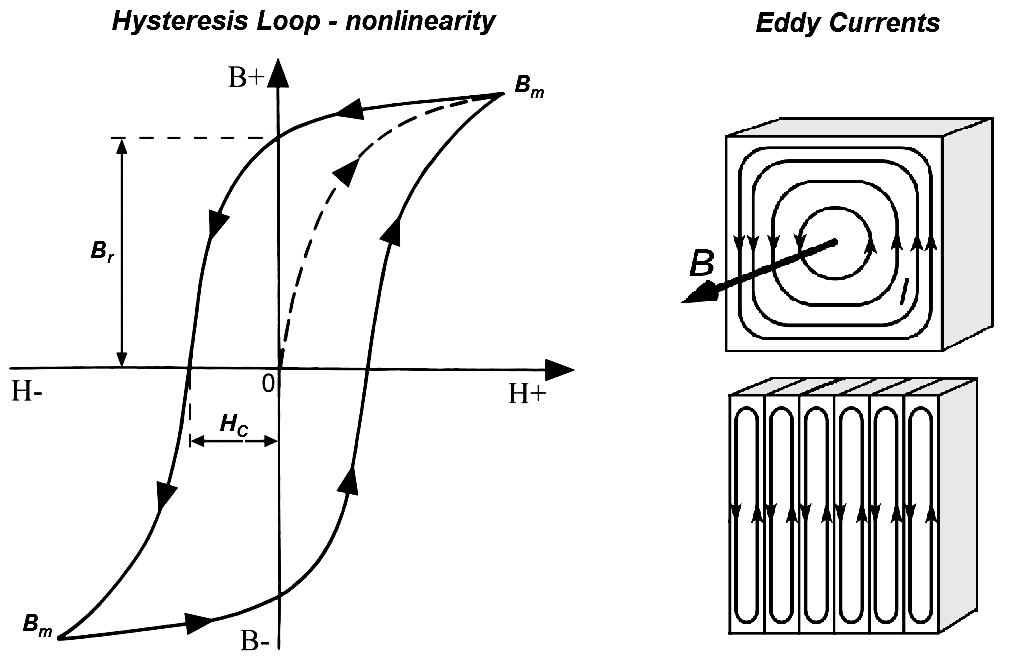
\includegraphics[scale=0.38]{obr08_smycka.png}
	\end{center}
  \end{frame}
%------------------------------------------------------------------------------
%Materials
%------------------------------------------------------------------------------
\section{\texorpdfstring{Materials}{Materials}}
%------------------------------------------------------------------------------
	\begin{frame}
	\frametitle{Metal magnetic materials}
	\textbf{Metal sheets (plates)}
	\begin{tabular}{m{0.6\linewidth} m{0.3\linewidth}}
		\begin{itemize}
		\item The most common type is rolled in warm state $\Rightarrow$ without any orientation of domains
	\end{itemize} 
	& 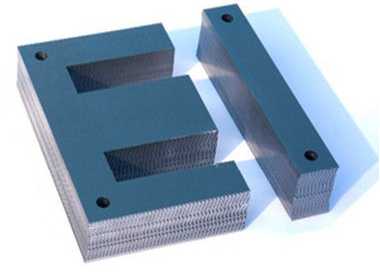
\includegraphics[scale=0.3]{obr09_zelezo.png}
	\end{tabular}
	\begin{tabular}{p{0.9\linewidth}}
	\begin{itemize}
		\item the cores with oriented texture are used for power applications - rolled sheets in cold state (better properties in defined direction)
		\item surface protection - insulation layer from oxide ($Fe_2O_3$), varnish, phosphate
	\end{itemize} 
	\end{tabular}
  \end{frame}
%------------------------------------------------------------------------------
	\begin{frame}
	\frametitle{Metal Glass}
	\begin{center}
		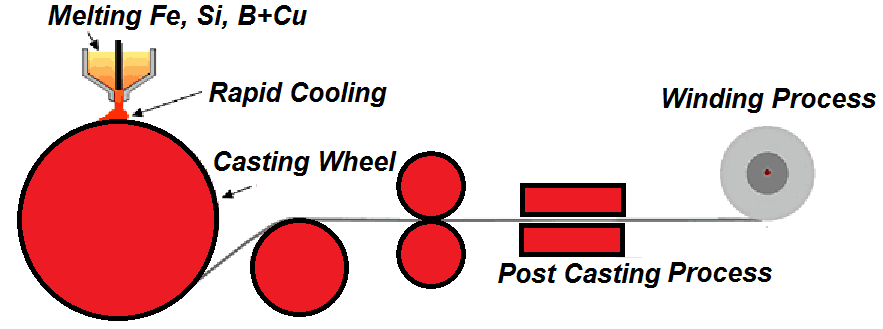
\includegraphics[scale=0.38]{obr10_amorfniKov.png}
	\end{center}
	
	\begin{itemize}
		\item materials without crystalline structure,
		\item production: very fast cooling of hot liquid alloy (melt), rolling into tin foils,
		\item properties: better than oriented sheets, low power losses, maximum of flux density $B$ higher than $2$~T
	\end{itemize}
  \end{frame}
%------------------------------------------------------------------------------
	\begin{frame}
	\frametitle{Powder Cores}
		\begin{tabular}{m{0.6\linewidth} m{0.3\linewidth}}
		\begin{itemize}
		\item \textbf{grains:} 1 $\mu$m to 10 $\mu$m pressed together with non-conductive binder, 
		\item low eddy currents up to HF but also low relative permeability ($\mu_r$ max. 100 or 200) .
	\end{itemize} 
	& 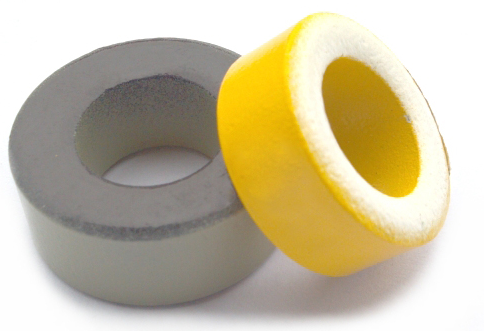
\includegraphics[scale=0.25]{obr11_zelezoprach.png}
	\end{tabular}
	\begin{tabular}{p{0.9\linewidth}}
	\begin{itemize}
		\item \textbf{binder:} polystyrene, bakelite or similar plastics
		\item \textbf{ferromagnetic grains:} silit, mumetal, AlSiFer, sendast, permalloy, the oldest materials based on iron+carbon
	\end{itemize} 
	\end{tabular}
  \end{frame}
%------------------------------------------------------------------------------
	\begin{frame}
	\frametitle{Ferrites}
		\begin{tabular}{m{0.6\linewidth} m{0.3\linewidth}}
		\begin{itemize}
		\item Sintered ceramic materials, mixture of metal oxides ($MeO + Fe_2O_3$) where \uv{$Me$} is: $Mn$, $Co$, $Cu$, $Zn$, $Ni$ 
		\item Ferrites are not conductive (semiconductors), there are no eddy currents
	\end{itemize} 
	& 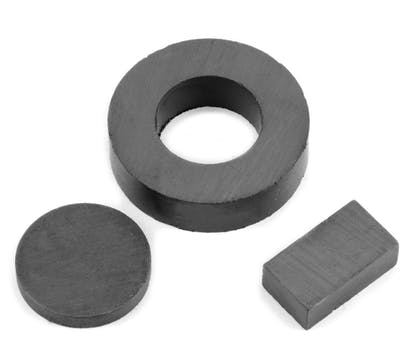
\includegraphics[scale=0.3]{obr12_ferrity.png}
	\end{tabular}
	\begin{tabular}{p{0.9\linewidth}}
	\begin{itemize}
		\item $B_{max}$ is very low, cca 0.3 T to 0.4 T; $\mu_{max}$ depends on composition, varies from 10 to 10 000, power losses ($D$-power dissipation factor) are very low $0.1\% -1\%$.
	\end{itemize} 
	\end{tabular}
  \end{frame}
%------------------------------------------------------------------------------
	\begin{frame}
	\frametitle{Ferrites - processing}
	
	\begin{itemize}
		\item Similar to common ceramics: mixing of oxides, pressing, drying, burning (co-firing), final sharpen into required shape.
		\item \textbf{Shapes: }
		
		\begin{itemize}
			\item enclosed cores: pots, EE, EI, UI, toroids;
			\item open cores: bars, tubes (pipes).
		\end{itemize}
		 
		\item \textbf{Properties:} very fragile and hard materials, low thermal transfer. Overheating and not proper assembly can cause mechanical damage.
		\item \textbf{Marking:} 
		\begin{itemize}
			\item N - Ni and Zn ferrites;
			\item H - Mn and Zn ferrites.
		\end{itemize}
	\end{itemize}
  \end{frame}
%------------------------------------------------------------------------------
	\begin{frame}
	\frametitle{Complex permeability of manganum-ferrites}
	\begin{center}
		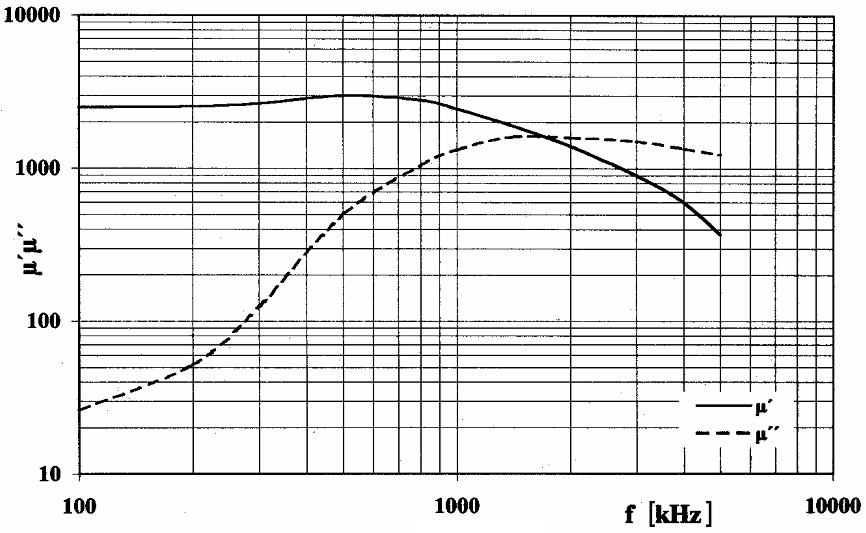
\includegraphics[scale=0.4]{obr13_permMnFerritu.png}
	\end{center}
  \end{frame}
%------------------------------------------------------------------------------
%Quality Factor
%------------------------------------------------------------------------------
\section{\texorpdfstring{Quality Factor}{Quality Factor}}
%------------------------------------------------------------------------------
	\begin{frame}
	\frametitle{Quality Factor}
	\small
	\begin{itemize}
		\item Q-factor describes amount of the losses in the inductance coil. Quality factor can be expressed as a ratio between reactive power $P_r$ and total active power $P_a$, which is dissipated in the inductor. It can be expressed by the equation:
		$$Q = \frac{P_r}{P_a}=\frac{\omega L}{R}$$
		\item Ideally Q factor increases linearly with frequency (coils without cores). The real characteristic is not linear due to the other factors like skin effect, permeability dependency and so on.
	\end{itemize}
	\begin{center}
		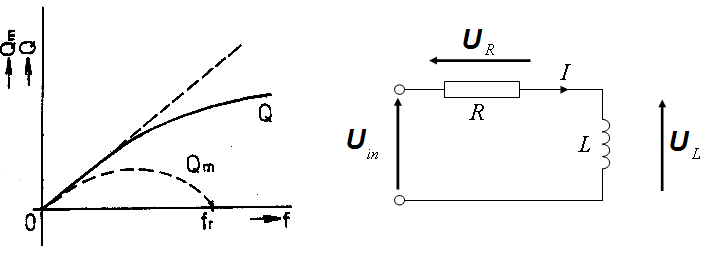
\includegraphics[scale=0.4]{obr14_cinjakosti.png}
	\end{center}
  \end{frame}
%------------------------------------------------------------------------------
	\begin{frame}
	\frametitle{Quality Factor - Air Core Example}
	\begin{center}
		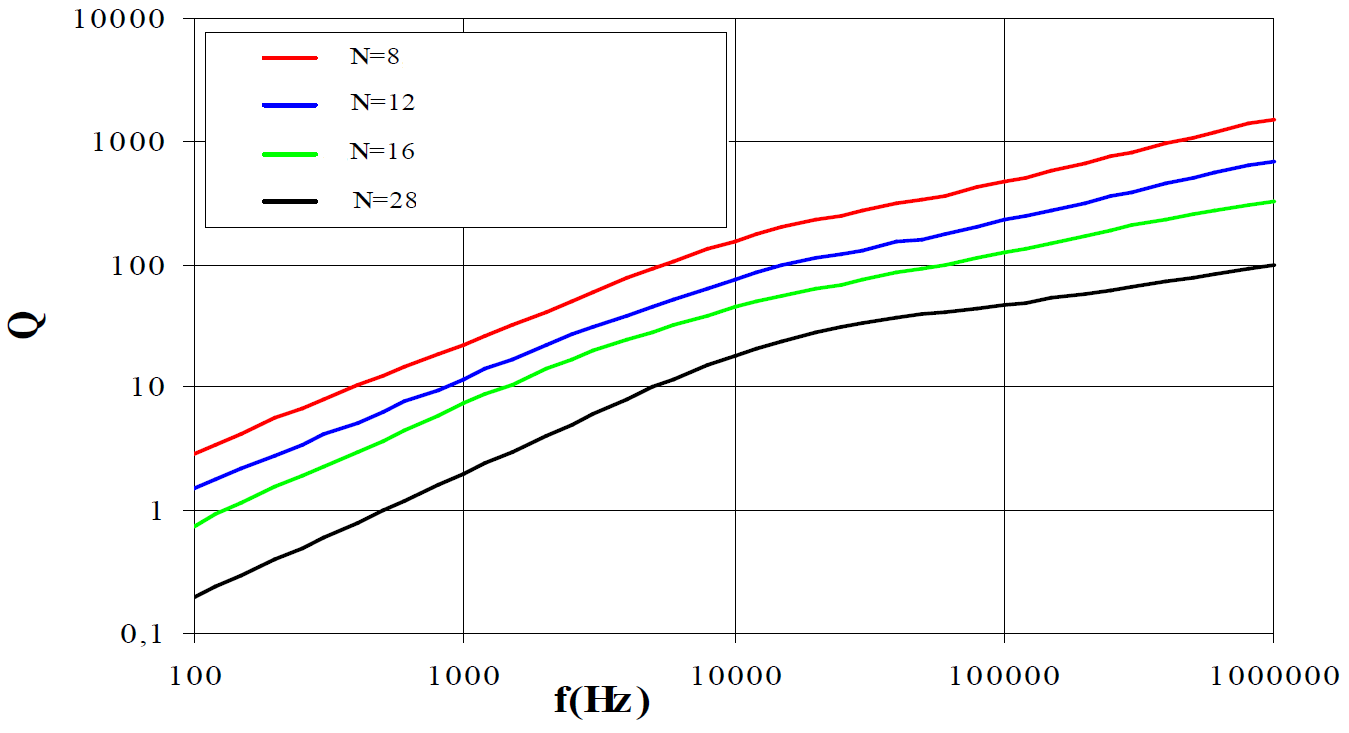
\includegraphics[scale=0.3]{obr15_qGraf.png}
	\end{center}
  \end{frame}
%------------------------------------------------------------------------------
\end{document}